\documentclass[11pt]{article}

% Anonymous review version. Switch to [final] after acceptance.
\usepackage[review]{acl}
\usepackage{times}
\usepackage{latexsym}
\usepackage[T1]{fontenc}
\usepackage[utf8]{inputenc}
\usepackage{microtype}
\usepackage{inconsolata}
\usepackage{graphicx}
\usepackage{booktabs}
\usepackage{pifont}
\usepackage{hyperref}

\newcommand{\cmark}{\ding{51}}
\newcommand{\xmark}{\ding{55}}
\newcommand{\pmark}{$\sim$}

\begin{document}
\title{Construct Validity Failures in Agentic AI Benchmarks:\\An Empirical Audit}

\author{Anonymous Authors}
% Anonymous submission for review. Uncomment for camera-ready:
% \author{Himaneesh Sompalle \\
%   Stonehill International School \\
%   Bengaluru, India \\
%   \texttt{himaneeshsompalle7@gmail.com}}

\begin{abstract}
Agent benchmarks are increasingly used to rank language models, guide procurement decisions, and set research priorities---yet what, exactly, do they measure? We apply construct validity analysis, drawn from psychometrics, to five major benchmarks spanning tool-use, code generation, and reasoning. Analyzing 15 models across these benchmarks, we find that cross-benchmark Spearman correlations are moderate at best (mean $\rho = 0.67$, range 0.10--0.92), 22\% of model pairs exhibit ranking inversions across benchmarks, and reasoning-specialized models (o1, o3-mini, o4-mini) that place in the top five on GPQA Diamond and MMLU-Pro drop to 6th--12th on tool-use benchmarks. The correlation between $\tau$-bench Airline and MMLU-Pro is 0.10 (bootstrap 95\% CI $[-0.87, 0.95]$, $n = 6$)---no evidence of a positive relationship---despite both being used to evaluate ``agent ability.'' These findings show that scores on these benchmarks do not induce a stable cross-benchmark model ranking and are consistent with multiple distinct underlying constructs rather than a unified ``agent ability''---making aggregate scores and single-number rankings misleading for the models and benchmarks practitioners consult today. We propose five desiderata for construct-valid agent evaluation and argue that benchmarks should report per-construct profiles rather than aggregate rankings.
\end{abstract}

\maketitle

\section{Introduction}
The proliferation of agent benchmarks has been remarkably rapid. In 2024--2025 alone, the community produced AgentBench~\cite{liu2024agentbench}, SWE-bench~\cite{jimenez2024swebench}, WebArena~\cite{zhou2024webarena}, GAIA~\cite{mialon2024gaia}, $\tau$-bench~\cite{yao2024taubench}, and BFCL~\cite{patil2025bfcl}, among others. Each claims to measure some aspect of ``agent ability''---a model's capacity to plan, use tools, navigate environments, write code, or converse with users over multiple turns.

These benchmarks now carry substantial weight. Leaderboard positions influence procurement decisions (``which model should we use for our agent pipeline?''), shape research priorities (``which capability gaps should we work on?''), and anchor marketing claims (``state-of-the-art agent performance''). Yet a fundamental question remains unexamined: do these benchmarks actually measure the constructs they claim to measure?

Consider a concrete scenario. A product team needs to select a model for a customer-service agent that handles refund requests, rebooks flights, and answers policy questions. They consult a composite leaderboard that ranks models by averaging SWE-bench, GPQA, and $\tau$-bench scores. The leaderboard recommends o4-mini, which ranks highly overall due to strong reasoning scores. But as we will show, o4-mini ranks 2nd on GPQA Diamond (reasoning) and 9th on $\tau$-bench Airline (the benchmark most similar to their use case)---a 7-rank discrepancy concealed by the aggregate score. The team deploys o4-mini, and their agent underperforms despite strong ``overall'' benchmark numbers. This is not a hypothetical; it is a predictable consequence of construct-invalid evaluation.

In psychometrics, this question is called \emph{construct validity}---the degree to which a test measures the theoretical construct it purports to measure~\cite{cronbach1955construct}. A valid IQ test should correlate with other IQ tests (convergent validity) and not correlate with personality tests (discriminant validity). A valid agent benchmark should similarly measure a well-defined capability, produce consistent rankings with other benchmarks measuring the same capability, and produce different rankings from benchmarks measuring different capabilities.

We apply this lens to the agent evaluation landscape. Our analysis covers five benchmarks---$\tau$-bench Retail, $\tau$-bench Airline, SWE-bench Verified, GPQA Diamond, and MMLU-Pro---evaluated on 15 models spanning frontier and mid-tier systems from OpenAI, Anthropic, and the open-weight ecosystem.

Our findings are concerning. Cross-benchmark correlations are moderate at best (mean $\rho = 0.67$), with some pairs showing no evidence of a positive relationship ($\rho = 0.10$, CI crossing zero). Roughly a fifth of model pairs (22\%) exhibit ranking inversions across benchmarks. Reasoning-specialized models that place at or near the top of GPQA Diamond and MMLU-Pro drop dramatically on tool-use benchmarks---yet both benchmark types are routinely cited as evidence of ``agent ability.'' These results indicate that scores on these benchmarks reflect multiple distinct constructs, and that ranking models on a single aggregate leaderboard lacks psychometric justification.

Our contributions are: (1)~To our knowledge, the first systematic construct validity analysis of agent benchmarks, applying psychometric methodology to a rapidly growing evaluation ecosystem (\S\ref{sec:method}). (2)~Empirical evidence that agent benchmark scores, as published, behave like measures of distinct capabilities: moderate cross-benchmark correlations, common ranking inversions, and a clear split between tool-use and reasoning constructs (\S\ref{sec:results}). (3)~Five desiderata for construct-valid agent evaluation that the community can adopt as benchmarks mature (\S\ref{sec:desiderata}).

\section{Background: Construct Validity in AI Evaluation}
\textit{Construct validity.} Introduced by Cronbach and Meehl~\cite{cronbach1955construct}, construct validity asks whether a test measures the theoretical attribute it claims to measure. A test has high construct validity when: (a)~it correlates with other tests of the same construct (convergent validity), (b)~it does not correlate with tests of unrelated constructs (discriminant validity), and (c)~its items internally cohere (internal consistency).

\textit{Prior critiques in NLP evaluation.} Schlangen~\cite{schlangen2021targeting} argued that NLP benchmarks often lack well-defined constructs, instead testing an undefined mix of abilities. Raji et al.~\cite{raji2021ai} showed that benchmark performance frequently fails to predict real-world utility. Bowman and Dahl~\cite{bowman2021what} warned against the ``benchmark treadmill'' where saturated benchmarks are replaced by harder ones without examining whether the measured construct has changed. Sompalle~\cite{evaleval} formalized these concerns for MCP tool-use evaluation, showing that prominent MCP benchmarks implicitly target divergent constructs without explicitly operationalizing them. The present work extends this line of critique to the agent evaluation domain, which has not yet received systematic psychometric scrutiny.

\textit{The agent benchmark landscape.} Current agent benchmarks vary widely in what they test. $\tau$-bench~\cite{yao2024taubench} evaluates tool-agent-user interaction in domain-specific scenarios (retail, airline), requiring multi-turn conversation and policy compliance. SWE-bench~\cite{jimenez2024swebench} tests code generation agents on real GitHub issues. GAIA~\cite{mialon2024gaia} tests multi-step question answering requiring web browsing and document parsing. GPQA Diamond~\cite{rein2024gpqa} tests graduate-level scientific reasoning. MMLU-Pro~\cite{wang2024mmlupro} tests broad knowledge across 14 academic domains. Despite measuring apparently different things, all are cited as evidence of ``model capability'' in aggregate leaderboards that rank models with a single composite score.

\section{Methodology}\label{sec:method}
\subsection{Benchmark Selection}
We select five benchmarks that span the agent evaluation landscape (Table~\ref{tab:benchmarks}).

\begin{table}[h]
\caption{Benchmarks analyzed, with claimed construct and task type.}
\label{tab:benchmarks}
\begin{tabular}{lll}
\toprule
Benchmark & Claimed construct & Type \\
\midrule
$\tau$-Retail & Tool-use + policy & Agent \\
$\tau$-Airline & Tool-use + policy & Agent \\
SWE-bench Verified & Code generation & Agent \\
GPQA Diamond & Scientific reasoning & Non-agent \\
MMLU-Pro & Broad knowledge & Non-agent \\
\bottomrule
\end{tabular}
\end{table}

We include two non-agent benchmarks (GPQA, MMLU-Pro) as discriminant validity controls. If agent benchmarks measure a construct distinct from ``general reasoning,'' they should correlate more strongly with each other than with GPQA or MMLU-Pro.

\subsection{Model Selection}
We collect published scores for 15 models spanning three capability tiers (Table~\ref{tab:models}).

\begin{table}[h]
\caption{Models analyzed, grouped by provider and tier.}
\label{tab:models}
\begin{tabular}{lll}
\toprule
Provider & Models & Tier \\
\midrule
Anthropic & Claude 3.5 Sonnet/Haiku, & Mid \\
 & Claude 3.7 Sonnet, & Frontier \\
 & Claude Sonnet/Opus 4, & Frontier \\
 & Claude Opus 4.1, & Frontier \\
 & Claude Sonnet 4.5 & Frontier \\
OpenAI & GPT-4o, GPT-4.5, & Mid \\
 & GPT-4.1/mini/nano, & Mid--Frontier \\
 & o1, o3-mini, o4-mini & Reasoning \\
\bottomrule
\end{tabular}
\end{table}

\textit{Score provenance and comparability.} All scores were recorded in May--June 2026 and re-verified against primary sources in July 2026. $\tau$-bench scores are taken from the Sierra Research leaderboard (as mirrored by llm-stats.com) and provider announcements, under the benchmark's standard configuration (pass\textasciicircum{}1, standard user simulator); $\tau$-bench results are known to be sensitive to the user-simulator model and agent scaffold, and third-party reproductions with modified simulators report different absolute scores, so we use only official-leaderboard and provider figures under the standard setting. SWE-bench Verified scores come from swebench.com and official model cards, using each provider's standard single-attempt agentic scaffold without parallel test-time compute (hence 77.2 for Claude Sonnet 4.5 rather than the 82.0 parallel-compute figure). GPQA Diamond scores come from provider launch announcements and model cards; Claude scores are without extended thinking, and o-series scores are at default reasoning effort (o3-mini at medium). MMLU-Pro scores come from official model cards and the MMLU-Pro leaderboard; prompting protocols vary somewhat across providers. We therefore cannot guarantee full cross-provider comparability within a column: providers self-report under nominally standard but not identically instrumented protocols. This residual protocol variance is itself a construct-validity concern---it motivates our desiderata D1 and D4---and it means our correlations should be read as properties of the published-score ecosystem that practitioners actually consult, not of a controlled experiment.

Not every model has been evaluated on every benchmark; we use pairwise-complete observations for correlation analyses, reporting sample sizes alongside each statistic.

Table~\ref{tab:scores} presents the complete cross-benchmark score matrix. Data availability varies: $\tau$-Retail has 100\% coverage (15/15 models), while $\tau$-Airline has 67\% (10/15). Models without published scores on a benchmark are excluded from pairwise analyses involving that benchmark.

\begin{table*}[t]
\caption{Cross-benchmark scores for 15 models. Scores are on native benchmark scales (0--100). Dashes indicate no published score. See \S3.2 for per-benchmark sources, dates, and evaluation configurations.}
\label{tab:scores}
\begin{tabular}{lccccc}
\toprule
Model & $\tau$-Retail & $\tau$-Airline & SWE-bench V. & GPQA Dia. & MMLU-Pro \\
\midrule
Claude 3.5 Sonnet & 69.2 & 46.0 & 49.0 & 65.0 & 78.0 \\
Claude 3.7 Sonnet & 81.2 & 58.4 & 62.3 & 68.0 & 78.2 \\
Claude Sonnet 4 & 80.5 & 60.0 & 72.7 & 75.4 & --- \\
Claude Opus 4 & 81.4 & 59.6 & 72.5 & 79.6 & --- \\
Claude Opus 4.1 & 82.4 & 56.0 & --- & --- & --- \\
Claude Sonnet 4.5 & 86.2 & 70.0 & 77.2 & 83.4 & --- \\
GPT-4o & 60.3 & --- & 33.2 & 53.6 & 72.6 \\
GPT-4.5 & 68.4 & 50.0 & 38.0 & 71.4 & 73.6 \\
GPT-4.1 & 68.0 & 49.4 & 54.6 & 56.5 & 73.6 \\
GPT-4.1 mini & 55.8 & --- & 28.9 & 43.7 & 64.2 \\
GPT-4.1 nano & 22.6 & --- & --- & --- & 55.6 \\
o1 & 70.8 & 50.0 & 48.9 & 78.0 & 83.6 \\
o3-mini & 57.6 & --- & 49.3 & 77.0 & 80.0 \\
o4-mini & 71.8 & 49.2 & 68.1 & 81.4 & 81.4 \\
Claude 3.5 Haiku & 51.0 & --- & 40.6 & 41.0 & 65.0 \\
\bottomrule
\end{tabular}
\end{table*}

\subsection{Analyses}
We conduct four analyses:

\textit{1.~Cross-benchmark rank correlations.} For each pair of benchmarks, we compute Spearman's $\rho$ on the models evaluated on both. If benchmarks measure the same construct, $\rho$ should be high ($> 0.85$); if they measure different constructs, it should be low.

\textit{2.~Convergent vs.\ discriminant validity.} We compare the mean correlation among agent benchmarks ($\tau$-Retail, $\tau$-Airline, SWE-bench) to the mean correlation between agent and non-agent benchmarks (GPQA, MMLU-Pro). Convergent validity requires within-agent correlations to exceed cross-domain correlations.

\textit{3.~Ranking inversions.} For each pair of benchmarks, we count how many model pairs swap ranking order. An inversion occurs when Model A scores higher than Model B on benchmark X, but lower on benchmark Y. High inversion rates indicate that rankings are benchmark-specific, not generalizable.

\textit{4.~Rank profile analysis.} For models with scores on 4+ benchmarks, we examine the spread of ranks across benchmarks. Because benchmarks rank different numbers of models ($\tau$-Airline $n{=}10$, $\tau$-Retail $n{=}15$), we percentile-normalize each rank to $[0,1]$ via $(\mathrm{rank}-1)/(n-1)$ (0 = best, 1 = worst) and report the percentile spread (max $-$ min). A model with a large percentile spread is ``construct-ambiguous'': its relative standing cannot be summarized by a single ranking.

\textit{Statistical considerations.} We use Spearman's rank correlation ($\rho$) rather than Pearson's $r$ because we are interested in ordinal relationships (rankings) rather than linear relationships between scores on different scales. For every pairwise $\rho$ we additionally report a percentile bootstrap 95\% confidence interval (10{,}000 resamples of the pairwise-complete model set). All significance tests use $\alpha = 0.05$. Because we conduct 10 pairwise comparisons, we note which results survive Bonferroni correction ($\alpha_{\mathrm{adj}} = 0.005$) in addition to the nominal threshold. Sample sizes for pairwise analyses range from 6 to 15; we flag all correlations computed on fewer than 8 observations as having limited statistical power, report them for completeness only, and base no headline claim solely on them.

\section{Results}\label{sec:results}
\subsection{Cross-Benchmark Correlations Are Moderate}
Figure~\ref{fig:heatmap} shows the pairwise Spearman correlation matrix. The mean correlation across all 10 benchmark pairs is $\rho = 0.67$---moderate, and well below the $\rho > 0.85$ threshold that would support a unified ``agent ability'' construct. The range is striking: from $\rho = 0.10$ ($\tau$-Airline $\times$ MMLU-Pro, $p = 0.85$, $n = 6$, bootstrap 95\% CI $[-0.87, 0.95]$) to $\rho = 0.92$ (GPQA $\times$ MMLU-Pro, $p < 0.001$, CI $[0.65, 1.00]$).

\begin{figure}[t]
\centering
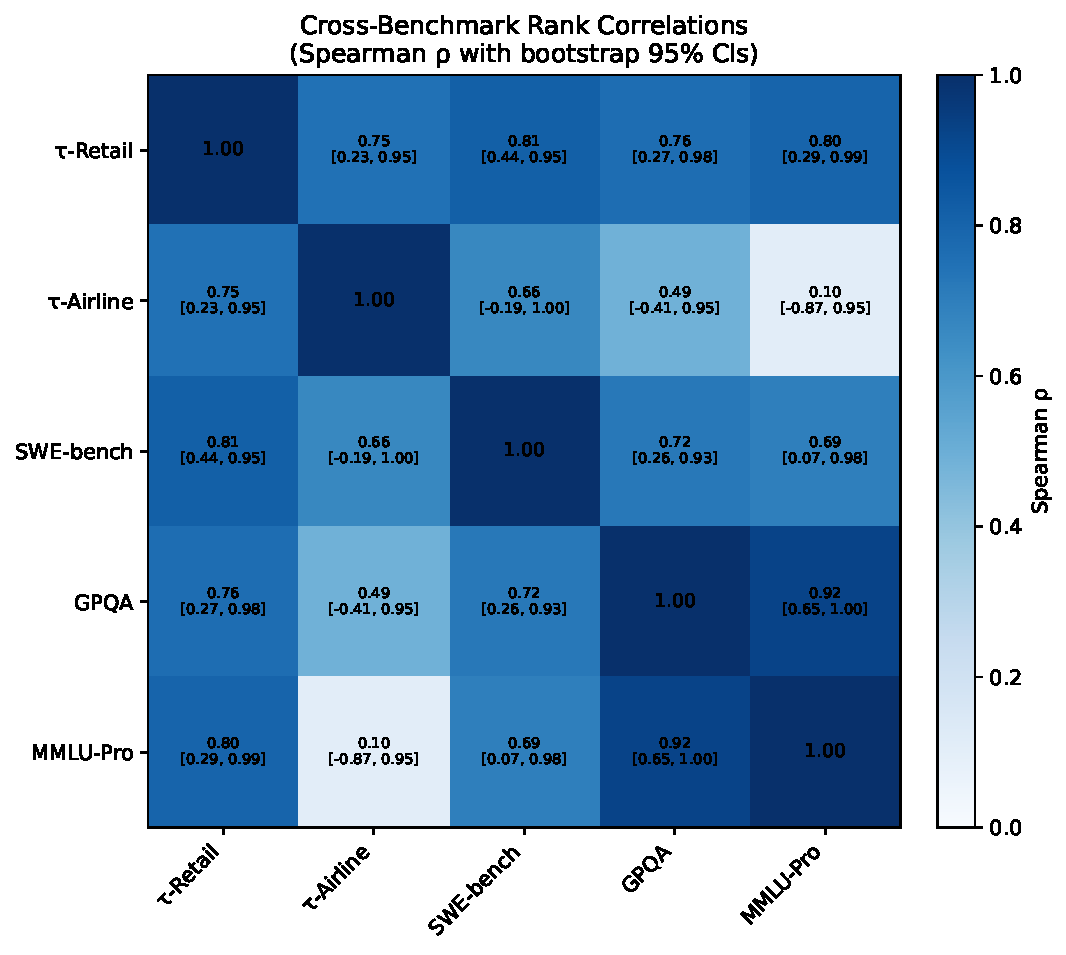
\includegraphics[width=\columnwidth]{fig1_heatmap.pdf}
\caption{Spearman rank correlations between benchmarks (pairwise complete, $n = 6$--$15$ per pair), with percentile bootstrap 95\% CIs (10{,}000 resamples) shown under each off-diagonal estimate. Correlations between $\tau$-Airline and the reasoning benchmarks are non-significant ($p > 0.05$), and their CIs are wide enough to include zero. The block structure suggests at least two latent factors: a ``tool-use'' cluster ($\tau$-Retail, $\tau$-Airline, SWE-bench) and a ``reasoning'' cluster (GPQA, MMLU-Pro), with $\tau$-Airline carrying most of the discriminant signal.}
\label{fig:heatmap}
\end{figure}

Within the agent cluster, correlations are moderate to high: $\tau$-Retail $\times$ SWE-bench $= 0.81$ $[0.44, 0.95]$, $\tau$-Retail $\times$ $\tau$-Airline $= 0.75$ $[0.23, 0.95]$, $\tau$-Airline $\times$ SWE-bench $= 0.66$ $[-0.19, 1.00]$. Within the reasoning cluster, GPQA $\times$ MMLU-Pro $= 0.92$ $[0.65, 1.00]$. Cross-domain correlations involving $\tau$-Airline are much lower: $\tau$-Airline $\times$ GPQA $= 0.49$ $[-0.41, 0.95]$ (non-significant, $n = 9$), $\tau$-Airline $\times$ MMLU-Pro $= 0.10$ $[-0.87, 0.95]$ (non-significant, $n = 6$). All intervals are percentile bootstrap 95\% CIs (10{,}000 resamples). The $\tau$-Airline intervals are especially wide and include zero; what they establish is the absence of evidence for a strong positive relationship, not a precise magnitude.

Notably, however, the discriminant signal is not uniform across the agent cluster. $\tau$-Retail correlates nearly as strongly with the reasoning benchmarks ($0.76$ with GPQA, $0.80$ with MMLU-Pro) as it does with the other agent benchmarks, suggesting that $\tau$-Retail behaves in part like a general-capability measure. The pattern therefore provides only partial evidence of convergent validity (mean within-agent $\rho = 0.74$ vs.\ mean cross-domain $\rho = 0.59$), with the separation between clusters driven mostly by $\tau$-Airline.

Even within the agent cluster, correlations are far from unity. $\tau$-Retail and $\tau$-Airline share the same framework, task structure, and evaluation protocol---they differ only in domain (retail vs.\ airline)---yet correlate at only $\rho = 0.75$. This suggests that domain-specific knowledge and policy understanding contribute substantially to performance, undermining the claim that either benchmark measures a domain-general ``tool-use ability.''

\subsection{Ranking Inversions Are Pervasive}
Table~\ref{tab:inversions} shows that ranking inversions occur in 22.1\% of model pairs on average.\footnote{In the absence of ties, the pairwise inversion rate equals $(1-\tau)/2$, where $\tau$ is Kendall\'s rank correlation; the two statistics are algebraically linked, so the inversion table and the Spearman matrix are complementary rather than independent evidence.} The rate is highest between $\tau$-Airline and the reasoning benchmarks (31--40\%), confirming that tool-use ability in the airline domain is only weakly related to reasoning ability.

\begin{table}[t]
\caption{Ranking inversion rates across all benchmark pairs. A higher rate means model rankings are less consistent between benchmarks.}
\label{tab:inversions}
\begin{tabular}{llrr}
\toprule
Benchmark A & Benchmark B & Inversions & Rate \\
\midrule
$\tau$-Retail & $\tau$-Airline & 10/45 & 22.2\% \\
$\tau$-Retail & SWE-bench & 14/78 & 17.9\% \\
$\tau$-Retail & GPQA & 14/78 & 17.9\% \\
$\tau$-Retail & MMLU-Pro & 9/55 & 16.4\% \\
$\tau$-Airline & SWE-bench & 8/36 & 22.2\% \\
$\tau$-Airline & GPQA & 11/36 & 30.6\% \\
$\tau$-Airline & MMLU-Pro & 6/15 & 40.0\% \\
SWE-bench & GPQA & 18/78 & 23.1\% \\
SWE-bench & MMLU-Pro & 10/45 & 22.2\% \\
GPQA & MMLU-Pro & 4/45 & 8.9\% \\
\midrule
\multicolumn{2}{l}{Mean across all pairs} & & 22.1\% \\
\bottomrule
\end{tabular}
\end{table}

Concrete examples of inversions illuminate the practical stakes: GPT-4.5 outperforms o3-mini on $\tau$-Retail (68.4 vs 57.6) but loses substantially on SWE-bench (38.0 vs 49.3). A team choosing a model for a tool-use pipeline would prefer GPT-4.5; a team choosing for code generation would prefer o3-mini. A single aggregate ranking would mislead at least one of them.

The inversions are not limited to cross-domain comparisons. Even within the agent benchmark cluster, GPT-4.1 beats o4-mini on $\tau$-Airline (49.4 vs 49.2) while losing on SWE-bench (54.6 vs 68.1)---a 14-point reversal on code generation despite near-identical tool-use scores. Claude Opus 4.1 ranks 2nd on $\tau$-Retail (82.4) but drops to 5th on $\tau$-Airline (56.0), despite both benchmarks using the same $\tau$-bench evaluation framework. This within-framework inversion is particularly concerning because it means that even a well-designed benchmark family cannot guarantee ranking stability across domains.

The inversion rate is also systematically higher when $\tau$-Airline is involved (22--40\%) compared to pairs not involving $\tau$-Airline (9--23\%), consistent with the correlation analysis suggesting $\tau$-Airline measures a partially distinct construct.

\subsection{Reasoning Specialization Does Not Transfer to Tool Use}
The most striking construct validity failure involves OpenAI's reasoning-specialized models. Figure~\ref{fig:scatter} visualizes the score relationships. o4-mini ranks \textbf{2nd} on GPQA Diamond (81.4\%) and \textbf{2nd} on MMLU-Pro (81.4\%), but drops to \textbf{6th} on $\tau$-Retail (71.8\%) and \textbf{9th} on $\tau$-Airline (49.2\%). o1 ranks \textbf{1st} on MMLU-Pro and 4th on GPQA, but 7th on $\tau$-Retail, 7th on $\tau$-Airline, and 9th on SWE-bench. o3-mini ranks 3rd on MMLU-Pro and 5th on GPQA but \textbf{12th} on $\tau$-Retail.

\begin{figure*}[t]
\centering
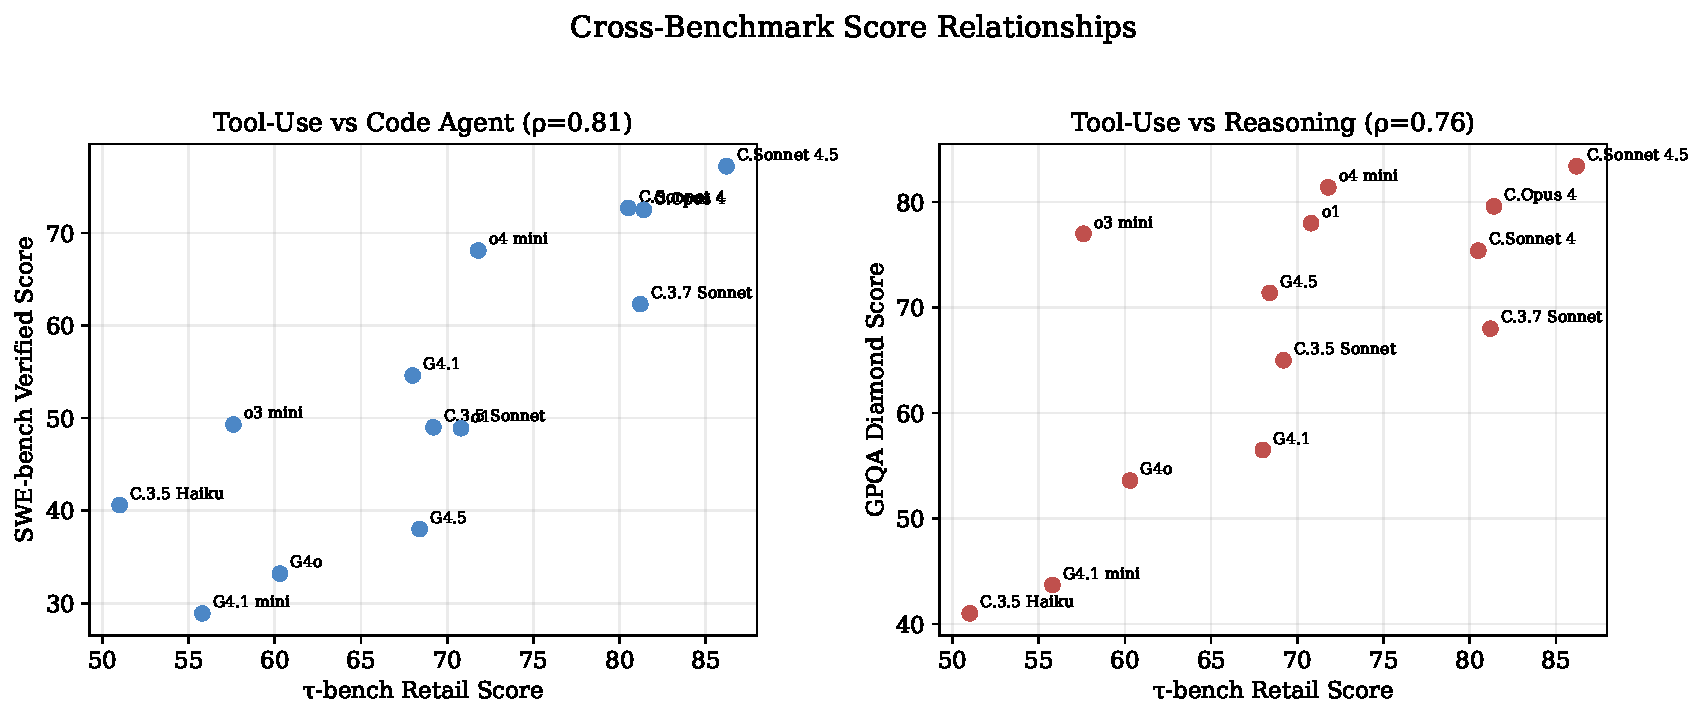
\includegraphics[width=0.95\textwidth]{fig2_scatter.pdf}
\caption{Score relationships between $\tau$-bench Retail and two other benchmarks. Left: tool-use vs.\ code agent scores are strongly correlated ($\rho = 0.81$), with Claude models clustering top-right. Right: tool-use vs.\ reasoning scores are also correlated ($\rho = 0.76$), but the o-series models (top-left region) rank highly on reasoning while placing mid-pack or lower on tool-use.}
\label{fig:scatter}
\end{figure*}

These models invest heavily in extended reasoning (chain-of-thought, test-time compute scaling), which dramatically improves performance on reasoning benchmarks. But sustained multi-turn tool-use with policy constraints---as tested by $\tau$-bench---appears to require a different capability profile that reasoning specialization does not provide.

Importantly, the dissociation is asymmetric. Reasoning specialization does not transfer to tool-use, but strong tool-use and strong reasoning are not mutually exclusive: Claude Sonnet 4.5 ranks 1st on all three agent benchmarks \emph{and} 1st on GPQA Diamond (83.4\%). The constructs are distinct---rank profiles differ substantially across models---but they are not anti-correlated. What the data rules out is not the possibility of a model excelling at both, but the assumption that excellence on one benchmark family predicts excellence on the other. Several earlier Claude models illustrate the same profile heterogeneity in the other direction: Claude 3.7 Sonnet ranks 4th on $\tau$-Retail but only 8th on GPQA.

Figure~\ref{fig:profiles} visualizes the complete rank profiles. The pervasive crossing of lines---particularly between the agent and reasoning columns---represents the central claim of this paper made visible: there is no stable ``model ranking'' that holds across benchmarks. Parallel lines would indicate that a single latent ability explains performance; the extensive crossing we observe is inconsistent with a uni-dimensional model.

\begin{figure*}[t]
\centering
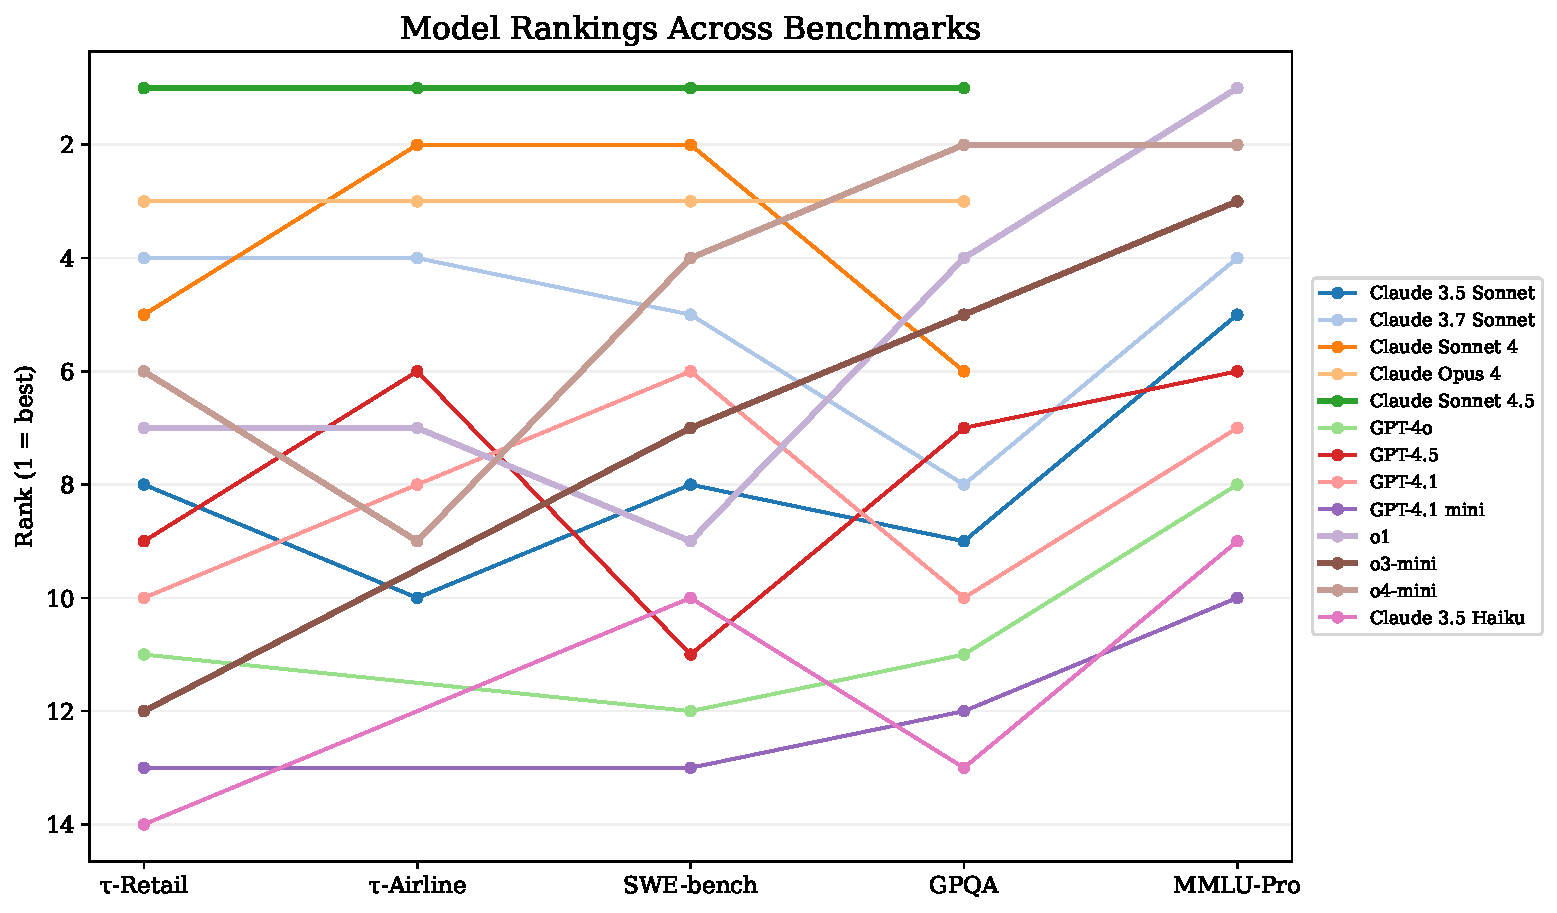
\includegraphics[width=0.92\textwidth]{fig3_profiles.pdf}
\caption{Model rank profiles across benchmarks. Each line traces one model's ranking (1 = best) from benchmark to benchmark. Parallel lines would indicate stable rankings; the extensive crossing visible here---especially between the agent benchmarks (left three columns) and reasoning benchmarks (right two columns)---confirms that rankings are benchmark-dependent. The o-series models (o1, o3-mini, o4-mini) show the most dramatic slope changes, rising sharply on reasoning benchmarks and falling on tool-use benchmarks; Claude Sonnet 4.5 is the notable exception, holding rank 1 on every benchmark on which it is scored.}
\label{fig:profiles}
\end{figure*}

The practical consequence is immediate. A practitioner consulting a composite leaderboard that averages these five benchmarks would get a ranking that is neither the tool-use ranking, nor the reasoning ranking, nor the code ranking---it would be an unprincipled mixture that misrepresents every model's actual capability profile.

\subsection{Rank Profiles Reveal Construct-Ambiguous Models}
Table~\ref{tab:spread} shows percentile-normalized rank spreads. After accounting for unequal field sizes, the reasoning-specialized models still dominate: o4-mini spans 81 percentile points (8th percentile on GPQA to 89th on $\tau$-Airline), o1 spans 67, and o3-mini spans 59. Raw ranks had overstated o3-mini's ambiguity (spread 9) relative to o4-mini (spread 7) because o3-mini's worst placement is on the larger $\tau$-Retail field; percentile normalization reverses that ordering. Any aggregate leaderboard that combines these benchmarks will misrepresent these models' capabilities to both their admirers and detractors.

\begin{table}[t]
\caption{Percentile-normalized rank profiles (0 = best in field, 100 = worst). Spread is max $-$ min percentile. Normalization uses $(\mathrm{rank}-1)/(n-1)$ so that ranks from unequal fields ($\tau$-Airline $n{=}10$, $\tau$-Retail $n{=}15$) are comparable. For contrast, the two most uniform profiles are shown below the rule.}
\label{tab:spread}
\small
\setlength{\tabcolsep}{3.5pt}
\begin{tabular}{lcccccc}
\toprule
Model & $\tau$-Ret. & $\tau$-Air. & SWE & GPQA & MMLU & Spread \\
\midrule
o4-mini & 36 & 89 & 25 & 8 & 10 & 81 \\
o1 & 43 & 67 & 67 & 25 & 0 & 67 \\
o3-mini & 79 & --- & 50 & 33 & 20 & 59 \\
GPT-4.5 & 57 & 56 & 83 & 50 & 50 & 33 \\
\midrule
Claude Opus 4 & 14 & 22 & 17 & 17 & --- & 8 \\
Claude Sonnet 4.5 & 0 & 0 & 0 & 0 & --- & 0 \\
\bottomrule
\end{tabular}
\end{table}

The Claude models, by contrast, remain comparatively uniform after normalization---Claude Opus 4 stays within an 8-point percentile band, and Claude Sonnet 4.5 is at percentile 0 on every benchmark on which it is scored. This does not mean Claude models are ``better'' in any absolute sense; it means their relative standing is less construct-ambiguous and therefore more predictable across deployment contexts.

\section{Desiderata for Construct-Valid Agent Benchmarks}\label{sec:desiderata}
Our analysis motivates five requirements that benchmark designers should satisfy before claiming to measure a well-defined agent capability.

\textit{D1: Explicit construct definition.} Every benchmark should state precisely what capability it measures and---equally important---what it does not measure. $\tau$-bench Retail does this relatively well: it explicitly tests tool-agent-user interaction under retail policy constraints, and its paper distinguishes between single-control and dual-control settings. Many other benchmarks are vaguer: AgentBench claims to test ``LLMs as agents'' across 8 environments without specifying which aspects of agency each environment isolates, making it impossible to know whether a score improvement reflects better planning, better tool use, or better instruction following.

\textit{D2: Convergent validity evidence.} If a benchmark claims to measure ``tool-use ability,'' it should demonstrate correlation ($\rho > 0.80$) with other established tool-use benchmarks. Our data shows that even $\tau$-Retail and $\tau$-Airline---which share the same evaluation framework, task structure, and metric---correlate at only 0.75, leaving roughly 44\% of the rank variance in one benchmark unexplained by the other ($1 - \rho^2 \approx 0.44$), likely attributable to domain-specific knowledge (retail policies vs.\ airline policies) rather than general tool-use ability. Benchmark papers should report cross-benchmark correlations as standard validation evidence, just as psychological test manuals report convergent validity coefficients.

\textit{D3: Discriminant validity evidence.} A tool-use benchmark should produce rankings that are \emph{different} from reasoning benchmarks. If they produce identical rankings, the tool-use benchmark is not measuring anything beyond general capability. Our finding that $\tau$-Airline $\times$ MMLU-Pro $= 0.10$ is encouraging from a discriminant validity perspective---it suggests $\tau$-Airline measures something genuinely distinct from broad knowledge---though the small overlapping sample ($n = 6$) means this estimate is imprecise. Conversely, $\tau$-Retail's high correlations with the reasoning benchmarks (0.76--0.80) suggest weaker discriminant validity. Either way, this should be demonstrated intentionally as part of benchmark validation, not discovered post hoc by external auditors.

\textit{D4: Per-construct score reporting.} Benchmarks with heterogeneous sub-tasks should report per-sub-task scores, not a single aggregate. Our analysis shows that $\tau$-Retail and $\tau$-Airline rankings diverge substantially; an aggregate $\tau$-bench score would obscure this divergence and mislead practitioners who care about one domain but not the other. Leaderboards should display \emph{capability profiles}---multi-column tables or radar charts showing performance on each sub-construct---rather than single composite numbers. This mirrors best practices in psychometrics, where intelligence tests report verbal, quantitative, and spatial sub-scores alongside any composite.

\textit{D5: Ranking stability disclosure.} Benchmark papers should report the expected ranking inversion rate with respect to related benchmarks. A benchmark where 40\% of model pairs invert relative to MMLU-Pro (as $\tau$-Airline does) should disclose this prominently, so practitioners know that MMLU-Pro rankings do not transfer to $\tau$-Airline performance. Concretely, we suggest benchmark papers include a table showing $\rho$ and inversion rate with at least three comparison benchmarks, analogous to the cross-validation tables standard in psychometric test manuals.

\subsection{Applying the Desiderata}
Table~\ref{tab:scorecard} applies our five desiderata to the benchmarks in this study. No benchmark satisfies all five, but $\tau$-bench comes closest: it defines its construct explicitly, publishes domain-specific scores, and $\tau$-Airline's discriminant profile is empirically strong. SWE-bench Verified satisfies D1 clearly (``resolve real GitHub issues'') but does not report cross-benchmark validation. GPQA and MMLU-Pro, as reasoning benchmarks, are not designed as agent evaluations but are routinely included in agent-focused composite leaderboards---a practice our analysis shows is problematic.

\begin{table}[h]
\caption{Desiderata scorecard. \cmark~= satisfied, \pmark~= partially, \xmark~= not satisfied. D1: explicit construct. D2: convergent validity. D3: discriminant validity. D4: per-construct scores. D5: stability disclosure.}
\label{tab:scorecard}
\begin{tabular}{lccccc}
\toprule
Benchmark & D1 & D2 & D3 & D4 & D5 \\
\midrule
$\tau$-Retail & \cmark & \xmark & \pmark & \cmark & \xmark \\
$\tau$-Airline & \cmark & \xmark & \pmark & \cmark & \xmark \\
SWE-bench & \cmark & \xmark & \xmark & \pmark & \xmark \\
GPQA & \cmark & \xmark & \xmark & \xmark & \xmark \\
MMLU-Pro & \pmark & \xmark & \xmark & \pmark & \xmark \\
\bottomrule
\end{tabular}
\end{table}

The striking preponderance of unmet criteria in Table~\ref{tab:scorecard} is not an indictment of any particular benchmark---it reflects the fact that construct validation is not yet standard practice in the AI evaluation community. Our proposal is that D1--D5 become part of the expected content of benchmark papers, analogous to how test-retest reliability and factorial structure are expected in psychometric test manuals.

\section{Discussion}
\textit{Implications for leaderboards and model selection.} Our findings directly challenge the practice of ranking models on composite leaderboards that aggregate scores across heterogeneous benchmarks. A composite score that averages $\tau$-Retail (tool-use), SWE-bench (code), and GPQA (reasoning) will systematically misrepresent models with non-uniform capability profiles---which, as we have shown, includes all reasoning-specialized models. We recommend that leaderboards adopt multi-dimensional displays (profiles per construct) rather than single-number rankings, and that model selection decisions be anchored to the specific benchmark most relevant to the deployment context. A team building a customer-service agent should prioritize $\tau$-bench scores; a team building a coding assistant should prioritize SWE-bench. Neither should rely on a composite that dilutes the signal they care about with benchmarks measuring unrelated capabilities.

\textit{Toward a construct map of agent capabilities.} Our correlation structure suggests at least two---and possibly three---distinct capability clusters. The first cluster, which we tentatively label \emph{structured tool-use}, encompasses $\tau$-Retail, $\tau$-Airline, and SWE-bench (mean within-cluster $\rho = 0.74$). These benchmarks all require multi-step tool interaction under constraints. The second cluster, \emph{academic reasoning}, includes GPQA and MMLU-Pro ($\rho = 0.92$). $\tau$-Airline may constitute the embryo of a third cluster, \emph{conversational persistence under policy constraints}, given its weak, non-significant correlations with the reasoning benchmarks and only moderate correlation with the other agent benchmarks. We emphasize that this clustering is tentative and requires confirmation with larger model sets and additional benchmarks; in particular, $\tau$-Retail's high correlations with the reasoning cluster show that the boundary between clusters is soft. Nonetheless, it provides an initial framework for organizing the rapidly expanding benchmark landscape.

\textit{What does $\tau$-Airline actually measure?} The near-zero point estimate between $\tau$-Airline and MMLU-Pro ($\rho = 0.10$, CI $[-0.87, 0.95]$, $n = 6$) and the weak, non-significant correlation with GPQA ($\rho = 0.49$) deserve further investigation. $\tau$-Airline tests an agent's ability to handle airline customer service interactions: rebooking flights, applying cancellation policies, and managing user frustration---all while following complex, domain-specific rules. Performance appears to depend on a capability profile that reasoning benchmarks capture only partially: the ability to maintain conversational coherence over many turns, apply domain rules consistently without hallucinating policy details, and recover gracefully from misunderstandings. This capability---which we might call ``situated policy compliance''---is critical for real-world agent deployments but has no established evaluation methodology outside of $\tau$-bench.

\textit{The ``g factor'' question.} In psychometrics, the debate over whether intelligence reduces to a single general factor ($g$) or multiple independent factors has a direct analog in AI evaluation. Our data suggests that ``agent ability'' does not reduce to a single factor: the correlation structure reveals at least two clusters with substantial unexplained variance between them. This multi-factor structure has implications for model development: improving reasoning (which helps GPQA) may not improve tool-use (which helps $\tau$-bench). The reasoning-specialized models (o1, o3-mini, o4-mini) are a natural experiment consistent with this: their architecture explicitly optimizes for extended reasoning, which produces dramatic improvements on GPQA and MMLU-Pro while leaving their tool-use rankings mid-pack. At the same time, the two factors are positively correlated rather than orthogonal, and Claude Sonnet 4.5's simultaneous first-place rank on both clusters shows that the factors can be jointly maximized---the analog of a model with both high verbal and high spatial sub-scores.

\textit{Limitations.} Our analysis faces several limitations, and our conclusions should be read as claims about the selected benchmarks, models, and published scores rather than about agent capability in general. First, the sample of 15 models, while spanning capability tiers and providers, is not exhaustive; open-weight models (Llama, Qwen, Mistral) are underrepresented due to limited benchmark coverage. Prior measurement-theoretic guidance for multi-trait benchmark validation recommends on the order of 20+ models for stable cross-benchmark correlation estimates~\cite{evaleval}; our pairwise samples of 6--15 fall short of that threshold, which is why we emphasize confidence intervals and treat the smallest pairs as directional rather than definitive. Second, not all models are evaluated on all benchmarks, requiring pairwise-complete analysis with varying sample sizes (6--15 per pair); the smallest pairs have limited statistical power, and the $\tau$-Airline correlations in particular should be interpreted cautiously. Third, we analyze published aggregate scores rather than per-task scores. Aggregate scores cannot separate item difficulty, domain knowledge, tool-use scaffolding, evaluator differences, and model-specific prompting effects from the latent capability of interest; our correlational evidence therefore constrains, but cannot identify, the underlying factor structure. Formally, what our data establishes is that the selected benchmark scores do not induce stable rankings across the selected models---a multi-factor capability structure is the most natural explanation, but confirming it requires item-level factor analysis. We note that our separate treatment of $\tau$-bench's retail and airline domains is itself a sub-task-level analysis of one benchmark family, and it revealed substantial within-family divergence; comparable decompositions of the other benchmarks require item-level data that is not currently published. Fourth, published scores are produced under heterogeneous evaluation protocols (e.g., reasoning-effort settings, extended-thinking modes, user-simulator models, scaffolds); we use each provider's standard single-attempt configuration where multiple figures exist, but residual protocol variance cannot be fully eliminated. Finally, our benchmark selection does not cover every major benchmark: GAIA, WebArena, OSWorld, and BFCL were excluded because, at data collection, too few of our 15 models had published scores on them under comparable configurations to support pairwise analysis. Whether the two-cluster structure persists when these benchmarks are added is an open empirical question; our released analysis code makes this straightforward to test as coverage grows.

{\sloppy
\textit{Reproducibility.} All benchmark scores used in this analysis are drawn from publicly available leaderboards (llm-stats.com, swebench.com) and official model cards, as recorded in May--June 2026 and re-verified against primary sources in July 2026. We release the complete cross-benchmark score matrix (Table~\ref{tab:scores}), correlation analysis code, and figure generation scripts.\footnote{Anonymized reproduction repository URL omitted for review; code and score matrix will be released upon acceptance.} We note that leaderboard scores are updated continuously as providers re-evaluate models; our analysis represents a snapshot, and we encourage replication on updated data. The pairwise-complete analysis methodology is robust to the addition of new models: adding a model requires only that it has been evaluated on at least two benchmarks.\par}

\section{Conclusion}
We have shown that, across five widely used benchmarks and 15 models, published scores do not induce a stable cross-benchmark model ranking. Cross-benchmark correlations are moderate (mean $\rho = 0.67$), ranking inversions affect 22\% of model pairs, and reasoning-specialized models exhibit dramatic rank drops on tool-use benchmarks. These results are inconsistent with a single latent ``agent ability'' factor underlying the selected benchmarks; a multi-factor structure of at least two positively correlated capability factors is the most natural explanation, though confirming it---and generalizing it beyond our benchmark and model sample---will require item-level data and broader coverage. Even under this appropriately cautious reading, the practical implications stand: aggregate leaderboards built from these scores are misleading, model selection should be benchmark-specific, and the community urgently needs construct-valid evaluation standards.

Our five desiderata---explicit construct definitions, convergent and discriminant validity evidence, per-construct reporting, and ranking stability disclosure---provide a concrete path forward. We have shown that no current benchmark satisfies all five, but the gap is practical rather than fundamental: the data and methods for construct validation already exist; what is needed is the expectation that benchmark papers include this analysis.

Looking forward, we see three priority actions. First, benchmark designers should publish item-level score matrices (models $\times$ tasks), not just aggregate scores, to enable the community to conduct independent factor analyses. Second, leaderboard maintainers should adopt multi-dimensional displays that show per-construct profiles rather than single composite rankings. Third, the evaluation community should develop a shared ``construct map'' of agent capabilities---a taxonomy of what distinct capabilities are required for different agent deployment contexts---to guide both benchmark design and model selection.

As agent benchmarks increasingly shape research priorities, procurement decisions, and public perception of AI progress, psychometric rigor is not optional. It is a prerequisite for trustworthy evaluation.

\bibliography{custom}
\end{document}
